\documentclass{beamer}
\geometry{papersize={10cm,20cm}}
\usetheme{Warsaw}
\usepackage{lmodern}
\usepackage{multirow}
\usepackage{caption}

\usepackage{amsmath}
\usepackage{amsfonts}
\usepackage{amssymb}
\usepackage{graphicx}
\begin{document}
\begin{frame}
		\begin{center}
			
	
{\bfseries \Huge OneClicq}\\

{\bfseries \LARGE Midhun Mk}\\
{\bfseries KMC18MCA007}
	\end{center}
\end{frame}

\begin{frame}
\section{Uml Diagrams}
\subsection{Activity Diagrams}

\begin{figure}[bph]
	\centering
	\includegraphics[width=1\linewidth, height=0.5\textheight]{C:/Users/Midhun/Pictures/ad/untitled_page}
	\caption{Vendor's Activity Diagram }
	\label{fig:untitledpage}
\end{figure}
\end{frame}

\begin{frame}

\begin{figure}[bph]
	\centering
	\includegraphics[width=1\linewidth, height=0.5\textheight]{C:/Users/Midhun/Pictures/adminnnnn/untitled_page}
	\caption{Admin's Activity Diagram}
	\label{fig:untitledpage}
\end{figure}
\end{frame}

\begin{frame}

\begin{figure}[bph]
	\centering
	\includegraphics[width=1\linewidth, height=0.5\textheight]{C:/Users/Midhun/Pictures/cus/untitled_page}
	\caption{Customer's Activity Diagram}
	\label{fig:untitledpage}
\end{figure}
\end{frame}



\begin{frame}
\subsection{Use Case Diagram}
\begin{figure}[bph]
	\centering
	\includegraphics[width=1\linewidth, height=0.7\textheight]{C:/Users/Midhun/Pictures/uml/untitled_page}
	\caption{Use Case Diagram of Admin, Vendor and Customer}
	\label{fig:untitledpage}
\end{figure}

\pagebreak
	
\end{frame}

\tiny 
\begin{frame}
	\section{User Story}
	\begin{center}
		\begin{tabular} { | p {0.3 cm} | p {1cm} | p {2 cm} |  p {4 cm} | }
			
			\hline\bf \vspace*{5pt} User story ID & \bf \vspace*{5pt}As a \textless Type of Users \textgreater & \bf \vspace*{5pt} I want to  \textless Perform	some task \textgreater &\bf \vspace*{5pt} So that I can \textless Achieve
			some goal \textgreater \\
			
			\hline
			1 & Admin & Home page & Home page for admin.\\ \hline
			2 & Admin & Login & Access to the system.\\ \hline
			3 & Vendor & Registering/Login &Vendor registering in to the vendor's portal the registered information will be provided to admin. \\ \hline
			4 & Admin
			& Approve/ Reject the vendor registeration 
			& The approval of vendor's registeration or rejecting of vendor's  registeration will be performed by the admin.\\ \hline
			
			5 &Vendor 
			& Add products to the system based on categories. 
			& Now the vendor will add the product to the system based on the categories after getting the approval from the admin.\\ \hline
			
			\hline
			6
			& Admin
			& Approve/Reject the product. 
			& The product added by the vendor now will be passed to the admin for the approval of placing in the site.\\ \hline
			
			
			7
			& Vendor
			& Delete/Update the product. 
			& Acting performing such as deletion or updation over the added products.\\ \hline
			
			8
			& Vendor
			& Add offer 
			& Adding offer to the products on certain occasion.\\ \hline
			
			
			9
			& Admin
			& Allow/ Reject the offer
			& If an offer is not valid then the admin can reject that offer. \\ \hline
			
			10
			& Vendor 
			& Earn coin 
			& The Customers can earn coins on basis of purchasing goods from the system.\\ \hline
			
			
			11
			& Customers
			& Login
			& Customers login into the system. \\ \hline
			
			12
			& Customers 
			& View 
			& View/Searching the product on the basis of categories.\\ \hline
			
			
			13
			& Customers
			& Add to cart 
			& Purchasing the product will redirect the add to cart page. 
			\\ \hline
			
			14
			& Customers
			& Rating  
			& Giving rating with feedback to the product. 
			\\ \hline
			
			15
			& Vendor 
			& Manage order 
			& Managing the order details(Report generation)\\ \hline
			
			
			16
			& Admin 
			& Manage user 
			& Managing the user details(Report generation)\\ \hline
			
			
			17
			
			& Admin 
			& Manage order
			& Managing the order details(Report generation)\\ \hline
			
			
		\end{tabular} 
		
		\vspace*{12pt}
	\end{center}

\end{frame}




\begin{frame}

\section{ Product Backlog}

\begin{center}
	\begin{tabular}{ | p {0.4 cm} | p {1.3 cm} | p {0.2 cm} |  p {0.5cm} |  p {1cm} |  p {1 cm} |  p {1.5 cm} | }
		
		\hline
		\centering	\bf USER STORY ID &
		\bf PRIORITY
		(LOW,HIGH,
		MEDIUM)   &
		\bf SIZE &
		\bf SPRINT & 
		\bf STATUS (PLANNED,
		PROGRESSED,
		COMPLETED) &
		\bf RELEASE DATE & 
		\bf RELEASE GOAL \\
		\hline
		
		1& HIGH & 6 & \multirow{8}{*}{1}&Completed   & 23-03-2021 &Home Page for Admin \\ \cline{1-3} \cline{5-7} 
		2& HIGH & 5 &                   &Completed   & 25-03-2021 &Access to the system  \\ \cline{1-3} \cline{5-7} 
		3& HIGH & 10 &                   &Completed   & 28-03-2021 &Vendor registering in
		to the vendor’s portal  \\ \cline{1-3} \cline{5-7} 
		4& HIGH & 7 &                   &Completed   & 31-03-2021 &Approval of vendor’s
		registeration \\ \cline{1-3} \cline{5-7} 
		
		5& HIGH & 10 &                   &Completed   & 2-04-2021 &Add the product to the
		system based  \\ \cline{1-3} \cline{5-7} 
		
		6& HIGH & 9 &                   &Completed   & 3-04-2021 &Approval of product\\ \cline{1-3} \cline{5-7} \hline
		
		
		7& LOW & 8 & \multirow{11}{*}{2}                   &Completed   & 06-04-2021 &Deletion or updation over product\\
		\cline{1-3} \cline{5-7}
		
		8& HIGH & 6 & &Completed   & 08-04-2021 &Adding offer to the
		products. \\ \cline{1-3} \cline{5-7} 
		9& High & 8 &                   &Completed   & 10-04-2021 & Allow/ Reject the offer	 \\ \cline{1-3} \cline{5-7} 
		10& HIGH & 6 &                   &Completed   &12-04-2021 &Customers earn coin\\
		\cline{1-3} \cline{5-7} 
		
		11& HIGH & 7 &                   &Completed   & 15-04-2021 &Customers login into
		the system.   \\ \cline{1-3} \cline{5-7}
		\hline                         
		
		12& MEDIUM & 9 & \multirow{10}{*}{3}&Completed   & 20-04-2021 &View/Searching the
		product on the basis of
		categories. \\ \cline{1-3} \cline{5-7} 
		13&HIGH & 9 & &Completed   & 23-4-2021 &Purchasing the product
		will redirect the add to
		cart page.\\ \cline{1-3} \cline{5-7}
		
		14& HIGH & 5 &                   &Completed   & 25-04-2021 &Giving rating with
		feedback to the product.\\ \cline{1-3} \cline{5-7} 
		
		15& HIGH & 6 &                   &Completed   & 29-04-2020 &Managing the order details(Vendor)\\ \cline{1-3} \cline{5-7}
		
		16&HIGH & 6 & &Completed   & 01-05-2021 &Managing the user details(Admin)\\ \cline{1-3} \cline{5-7}
		
		17& HIGH & 5 &                   &Completed   & 03-05-2021 &Managing the order details(Admin)\\ \cline{1-3} \cline{5-7} 
		\hline   
		
		
	\end{tabular}
	
\end{center}	
\end{frame}
\begin{frame}
	\section{ Sprint Backlog}
	
	\begin{figure}[bph]
		\centering
		\includegraphics[width=0.7\linewidth, height=0.4\textheight]{C:/Users/Midhun/Pictures/sprintback/s1}
		
		
	\end{figure}
	
	
	
	\begin{figure}[bph]
		\centering
		\includegraphics[width=0.7\linewidth]{C:/Users/Midhun/Pictures/sprintback/s2}
		
	\end{figure}
	
	\pagebreak
\end{frame}
\begin{frame}
	
	\begin{figure}[bph]
		\centering
		\includegraphics[width=0.7\linewidth, height=0.4\textheight]{C:/Users/Midhun/Pictures/sprintback/s3}
		\includegraphics[width=0.7\linewidth]{C:/Users/Midhun/Pictures/sprintback/s4}
		
	\end{figure}
	
	\pagebreak
	\begin{figure}[bph]
		\centering
		\includegraphics[width=0.7\linewidth, height=0.4\textheight]{C:/Users/Midhun/Pictures/sprintback/s5}
		
		
	\end{figure}
\end{frame}
\begin{frame}

	\pagebreak
	\begin{figure}[bph]
		\centering
		\includegraphics[width=0.7\linewidth, height=0.4\textheight]{C:/Users/Midhun/Pictures/sprintback/s6}
		
		
	\end{figure}
	\pagebreak
	\begin{figure}[bph]
		\centering
		\includegraphics[width=0.7\linewidth, height=0.4\textheight]{C:/Users/Midhun/Pictures/sprintback/s7}
		
		
	\end{figure}
	\pagebreak
\end{frame}	
	
	\begin{frame}
		
	
	\begin{figure}[bph]
		\centering
		\includegraphics[width=0.7\linewidth, height=0.4\textheight]{C:/Users/Midhun/Pictures/sprintback/s8}
		
		
		\caption{Sprint Backlog}
		
	\end{figure}
	
\end{frame}	




	\begin{frame}

\section{Database Design}
\subsection{Admin}

\begin{center}
	\begin{tabular} { | p {0.2 cm} | p {1 cm} | p {1.5 cm} |  p {1 cm} |  p {3 cm} | }
		
		\hline
		\centering	\bf No. &
		\bf Name & 
		\bf Type & 
		\bf Constraints & 
		\bf Description \\
		\hline
		\centering	1 &id &  int(20) & Primary key & Id no\\ \hline	
		\centering	2 & name & Varchar(80) & Not Null & Name of admin\\ \hline	\centering	3 & email & Varchar(100) & Not Null & Email-Id of admin\\ \hline
		\centering 4 & mobile & varchar(20) & Not Null &Mobile no of admin\\ \hline
		\centering 5 & password & varchar(100) & Not Null & Password of admin \\ \hline
		\centering 5 & isAdmin & tinyiny(1) & Not Null & To check wether admin or not\\ \hline
	\end{tabular}
	\vspace*{12pt}
	\captionof{table}{Table of Admin}
\end{center}



\subsection{Banners}

\begin{center}
	\begin{tabular} { | p {0.2 cm} | p {1 cm} | p {1.5 cm} |  p {1 cm} |  p {3 cm} | }
		
		\hline
		\centering	\bf No. &
		\bf Name & 
		\bf Type & 
		\bf Constraints & 
		\bf Description \\
		\hline
		\centering	1 &id & int(11)   & Primary key &Product's id\\ \hline	
		\centering	2 &productname  & varchar(100)  & Not Null & Product's name \\ \hline	
		\centering	3 & image &varchar(100) & Not Null & Product's image\\ \hline
		
	\end{tabular}
	\vspace*{12pt}
	\captionof{table}{ Table of Banners}
\end{center}

\subsection{Brands}

\begin{center}
	\begin{tabular} { | p {0.2 cm} | p {1 cm} | p {1.5 cm} |  p {1 cm} |  p {3 cm} | }
		
		\hline
		\centering	\bf No. &
		\bf Name & 
		\bf Type & 
		\bf Constraints & 
		\bf Description \\
		\hline
		\centering	1 &id  & bigint(20)	  & Primary key &Brand id\\ \hline	
		\centering	2 &name  & varchar(255) & Not Null &Image of brand \\ \hline	
		\centering	3 &logo  & varchar(250) & Not Null & Logo of brand\\ \hline
		
	\end{tabular}
	\vspace*{12pt}
	\captionof{table}{Table of Brands}
\end{center}


\subsection{Business types}

\begin{center}
		\begin{tabular} { | p {0.2 cm} | p {1 cm} | p {1.5 cm} |  p {1 cm} |  p {3 cm} | }
			
		\hline
		\centering	\bf No. &
		\bf Name & 
		\bf Type & 
		\bf Constraints & 
		\bf Description \\
		\hline
		\centering	1 & id&  bigint(20)  & Primary key &Business type's id\\ \hline	
		\centering	2 &  name& varchar(50)  & Not Null & Business type's name \\ \hline	
		\centering	3 &  active& tinyint(1)& Not Null &To check wether business type is active or not \\ \hline
		
	\end{tabular}
	\vspace*{12pt}
	\captionof{table}{Table of Business types}
\end{center}


\subsection{Carts}

\begin{center}
		\begin{tabular} { | p {0.2 cm} | p {1 cm} | p {1.5 cm} |  p {1 cm} |  p {3 cm} | }
			
		\hline
		\centering	\bf No. &
		\bf Name & 
		\bf Type & 
		\bf Constraints & 
		\bf Description \\
		\hline
		\centering	1 &id &  bigint(20) & Primary key & Cart's id\\ \hline	
		\centering	2 & productid & bigint(20)  & Not Null & Product's id \\ \hline	
		\centering	3 & userid &bigint(20) & Not Null & User's id\\ \hline
		\centering 4 & mrp & varchar(55) & Not Null & MRP of product\\ \hline
		\centering 5 & price & varchar(55) & Not Null & Price of product\\ \hline
		\centering 6 & units &  int(11)& Not Null & Number of product\\ \hline
		\centering 7 & dqpoint &varchar(55)   & Not Null & Dairy Queen points\\ \hline
		
		\centering 10 & pgst &  float(8,2) & Not Null & GST of product \\ \hline
		\centering 11 & poffer & varchar(55)  & Not Null & Offer on product \\ \hline
		\centering 12 & pcategoryid & varchar(55) & Not Null & Product category id \\ \hline
		\centering 13 & pbrandid & varchar(55) & Not Null & Product brand id \\ \hline
		
	\end{tabular}
	\vspace*{12pt}
	\captionof{table}{Table of Carts}
\end{center}

\end{frame}	

\begin{frame}
	
	
	\subsection{Categories}
	
	\begin{center}
		\begin{tabular} { | p {0.2 cm} | p {1 cm} | p {1.5 cm} |  p {1 cm} |  p {3 cm} | }
				
			\hline
			\centering	\bf No. &
			\bf Name & 
			\bf Type & 
			\bf Constraints & 
			\bf Description \\
			\hline
			\centering	1 &id &  bigint(20) & Primary key & Category's id\\ \hline	
			\centering	2 & name & varchar(200) & Not Null &Category name \\ \hline	
			\centering	3 & description &varchar(200) & Not Null & Category Description\\ \hline
			\centering 4 & image & varchar(510)  & Not Null &Category image\\ \hline
			\centering 5 & commission & varchar(150)  & Not Null &Commision for admin based on product \\ \hline
		\end{tabular}
		\vspace*{12pt}
		\captionof{table}{Table of Categories}
	\end{center}
	
	
	\subsection{Sub categories}
	
	\begin{center}
			\begin{tabular} { | p {0.2 cm} | p {1 cm} | p {1.5 cm} |  p {1 cm} |  p {3 cm} | }
				
			\hline
			\centering	\bf No. &
			\bf Name & 
			\bf Type & 
			\bf Constraints & 
			\bf Description \\
			\hline
			\centering	1 &id &  bigint(20) & Primary key & Sub Category's id\\ \hline	
			\centering	2 & name & varchar(200) & Not Null & Sub Category name \\ \hline	
			\centering	3 & category id &bigint(20)  & Not Null & Category id\\ \hline
		\end{tabular}
		\vspace*{12pt}
		\captionof{table}{Table of sub Categories}
	\end{center}
	
	
	
	
	
	
	\subsection{Delivery addresses}
	
	\begin{center}
	\begin{tabular} { | p {0.2 cm} | p {1 cm} | p {1.5 cm} |  p {1 cm} |  p {3 cm} | }
			
			\hline
			\centering	\bf No. &
			\bf Name & 
			\bf Type & 
			\bf Constraints & 
			\bf Description \\
			\hline
			\centering	1 &id & int(20)  & Primary key &Delivery address's id\\ \hline	
			\centering	2 &  userid& bigint(20) & Not Null & Customer's id\\ \hline	
			\centering	3 & name & varchar(100)& Not Null & Customer's name \\ \hline
			\centering 4 & mobile &  VARCHAR(20) & Not Null &Customer's mobile no\\ \hline
			\centering 5 & email & varchar(200) & Not Null & Customer's email id\\ \hline
			\centering 6 &pincode  & int(11) & Not Null & Customer's pincode\\ \hline
			\centering 7 & address & VARCHAR(200) & Not Null &Customer's address \\ \hline
			\centering 8 & city &  varchar(50)& Not Null &Customer's city \\ \hline
			\centering 9 & state & varchar(50) & Not Null & Customer's state\\ \hline
			
		\end{tabular}
		\vspace*{12pt}
		\captionof{table}{Table of Delivery Address}
	\end{center}
	
	
	
	\subsection{Discounts}
	
	\begin{center}
		\begin{tabular} { | p {1 cm} | p {3 cm} | p {3 cm} |  p {3 cm} |  p {3 cm} | }
			
			\hline
			\centering	\bf No. &
			\bf Name & 
			\bf Type & 
			\bf Constraints & 
			\bf Description \\
			\hline
			\centering	1 &id &   & Primary key &Discount's id\\ \hline	
			\centering	2 &productid  &bigint(20)   & Not Null & Product's id \\ \hline	
			\centering	3 & categoryid & bigint(20) & Not Null & Category's id\\ \hline
			\centering 4 & vendorid & bigint(20)  & Not Null &Vendors's id\\ \hline
			\centering 5 & brandid & bigint(20)  & Not Null &Brand's id \\ \hline
			\centering 6 &offerprice  &  double& Not Null & Offer price\\ \hline
			\centering 7 & offerpercentage &  double& Not Null &Offer percentage \\ \hline
			\centering 8 & validfrom &  datetime& Not Null & Validity from\\ \hline
			\centering 9 &validto  &  datetime& Not Null & Validity to\\ \hline
			
		\end{tabular}
		\vspace*{12pt}
		\captionof{table}{Table of Discounts}
	\end{center}
	
	
	
		
\end{frame}	



\begin{frame}	
\subsection{Orders}

\begin{center}
	\begin{tabular} { | p {0.2 cm} | p {1 cm} | p {1.5 cm} |  p {1 cm} |  p {3 cm} | }
		
		\hline
		\centering	\bf No. &
		\bf Name & 
		\bf Type & 
		\bf Constraints & 
		\bf Description \\
		\hline
		\centering	1 & id&  bigint(20) & Primary key &Order's id\\ \hline	
		\centering	2 & orderrefnumber & varchar(500) & Not Null & Order reference number\\ \hline	
		\centering	3 & vendorid &bigint(20) & Not Null & Vendor's id\\ \hline
		\centering 4 & productid &  bigint(20)& Not Null &Product's id\\ \hline
		\centering 5 & customerid & bigint(20) & Not Null &Customer's id \\ \hline
		\centering 6 &  paymentmethod&  bigint(20)& Not Null & Payment methods \\ \hline
		\centering 7 &  orderat& timestamp & Not Null & When was order placed\\ \hline
		\centering 8 &  shippingaddressid&   bigint(20) & Not Null & Shipping address id \\ \hline
		\centering 9 &  billingaddressid&   bigint(20) & Not Null & Billing address id\\ \hline
		\centering 10 &  total& decimal(15,8)  & Not Null & Total amount \\ \hline
		
	\end{tabular}
	\vspace*{12pt}
	\captionof{table}{Table of Orders}
\end{center}



\subsection{OTPS}

\begin{center}
	\begin{tabular} { | p {0.2 cm} | p {1 cm} | p {1.5 cm} |  p {1 cm} |  p {3 cm} | }
		
		\hline
		\centering	\bf No. &
		\bf Name & 
		\bf Type & 
		\bf Constraints & 
		\bf Description \\
		\hline
		\centering	1 &id &  bigint(20)  & Primary key & OTP's id\\ \hline	
		\centering	2 & mobile &  varchar(191) & Not Null & Mobile no to which otp is send\\ \hline	
		\centering	3 & otp &varchar(191) & Not Null & OTP number\\ \hline
		
	\end{tabular}
	\vspace*{12pt}
	\captionof{table}{Table of OTP}
\end{center}



\subsection{Point Malls}

\begin{center}
	\begin{tabular} { | p {0.2 cm} | p {1 cm} | p {1.5 cm} |  p {1 cm} |  p {3 cm} | }
		
		\hline
		\centering	\bf No. &
		\bf Name & 
		\bf Type & 
		\bf Constraints & 
		\bf Description \\
		\hline
		\centering	1 &id &  bigint(20) & Primary key &Point's id\\ \hline	
		\centering	2 & userid &  bigint(20)& Not Null & User's id \\ \hline	
		\centering	3 & productid &bigint(20) & Not Null &Product's id \\ \hline
		\centering 4 &  points	& int(50)  & Not Null & Points\\ \hline
		
	\end{tabular}
	\vspace*{12pt}
	\captionof{table}{Table of Point Malls}
\end{center}





\end{frame}
\begin{frame}

\subsection{Vendor}

\begin{center}
	\begin{tabular} { | p {0.2 cm} | p {1 cm} | p {1.5 cm} |  p {1 cm} |  p {3 cm} | }
		
		\hline
		\centering	\bf No. &
		\bf Name & 
		\bf Type & 
		\bf Constraints & 
		\bf Description \\
		\hline
		\centering	1 &id & int(10)   & Primary key &Vendor's id\\ \hline	
		\centering	2 & 	name & varchar(25) & Not Null &Vendor's name \\ \hline	
		\centering	3 & 	mob & varchar(25)& Not Null & Vendor's mobile no\\ \hline
		\centering 4 & email &  varchar(25)& Not Null &Vendor's email\\ \hline
		\centering 5 &pass  & varchar(25) & Not Null &Vendor's password \\ \hline
		\centering  6& regstatus & varchar(25) & Not Null & Vendor's registeration status\\ \hline
		\centering  7&companyname  & varchar(25) & Not Null &Vendor's company name \\ \hline
		\centering  8&	officeno  & int(10) & Not Null & Vendor's office no\\ \hline
		\centering 9& state &varchar(25)  & Not Null &Vendor's state \\ \hline
		\centering  10&district  & varchar(25) & Not Null & Vendor's district\\ \hline
		\centering  11& location & varchar(25) & Not Null & Vendor's location\\ \hline
		\centering  12& businesstype & varchar(25) & Not Null &Vendor's business type \\ \hline
		\centering  13& tradelicenceno & int(10)  & Not Null &Trade licence number \\ \hline
		\centering  14&	tradedocument  & varchar(50) & Not Null & Trade document \\ \hline
		\centering  15& shipping & varchar(25) & Not Null &Vendor's shipping mode \\ \hline
		\centering  16& gstno &  varchar(25)& Not Null & Vendor's GST no.\\ \hline
		\centering  17&	panno& varchar(25) & Not Null & PAN number\\ \hline
		\centering  18&	fssaino	&  varchar(25)& Not Null & FSSAI number\\ \hline
		\centering 19 &	vendorname	  &  varchar(25)& Not Null & Vendor full name  \\ \hline
		\centering  20& accounttype	 &varchar(25)  & Not Null & Bank account type \\ \hline
	\end{tabular}
	\vspace*{12pt}
	\captionof{table}{Table of Vendor}
\end{center}



\end{frame}	

\begin{frame}
	
	\subsection*{Vendor(Remaining..)}
	
	\begin{center}
	\begin{tabular} { | p {0.2 cm} | p {1 cm} | p {1.5 cm} |  p {1 cm} |  p {3 cm} | }
			
			\hline
			\centering	\bf No. &
			\bf Name & 
			\bf Type & 
			\bf Constraints & 
			\bf Description \\
			\hline
			
			
			
			
			
			\centering  21&  storename&  varchar(25)& Not Null & Store name \\ \hline
			\centering  22& sellingcat	 &varchar(25)  & Not Null & Selling categories\\ \hline
			\centering  23&pandocument	  &varchar(25)  & Not Null & PAN Documents\\ \hline
			\centering  24&	adminstatus  &varchar(20)  & Not Null & Admin status\\ \hline
			\centering  25& signature & varchar(25) & Not Null & Vendor's signature \\ \hline
			\centering  26&cancelledcheque  & varchar(25) & Not Null & Cancelled cheque\\ \hline
			\centering  27&	ifsccode  &varchar(25)  & Not Null &IFSC code \\ \hline
			\centering  28&	accountno  & varchar(25) & Not Null & Bank account number\\ \hline
			\centering  29& 	nameinbank	 &  varchar(25)& Not Null & Name in bank document\\ \hline
			\centering  30& gstdocument	 &  varchar(25)& Not Null & GST document \\ \hline
			\centering  31& 	iddocument	 &  varchar(25)& Not Null &Id Document \\ \hline
			\centering  32& storelogo & varchar(25) & Not Null & Store's logo\\ \hline
			
		\end{tabular}
		\vspace*{12pt}
		\captionof{table}{Table of Vendor}
	\end{center}
	
	\subsection{Vendor Categories}
	
	\begin{center}
	\begin{tabular} { | p {0.2 cm} | p {1 cm} | p {1.5 cm} |  p {1 cm} |  p {3 cm} | }
			
			\hline
			\centering	\bf No. &
			\bf Name & 
			\bf Type & 
			\bf Constraints & 
			\bf Description \\
			\hline
			\centering	1 &id & bigint(20)   & Primary key & Vendor category's id\\ \hline	
			\centering	2 & vendorid &  bigint(20) & Not Null &Vendor's id \\ \hline	
			\centering	3 & categoryid &bigint(20) & Not Null & Category id\\ \hline
		\end{tabular}
		\vspace*{12pt}
		\captionof{table}{Table of Vendor Categories}
	\end{center}
	
	\newpage 
	\subsection{Wish List}
	
	\begin{center}
	\begin{tabular} { | p {0.2 cm} | p {1 cm} | p {1.5 cm} |  p {1 cm} |  p {3 cm} | }
			
			\hline
			\centering	\bf No. &
			\bf Name & 
			\bf Type & 
			\bf Constraints & 
			\bf Description \\
			\hline
			\centering	1 &id &  bigint(20) & Primary key &Wish list's id\\ \hline	
			\centering	2 & userid & bigint(20) & Not Null & User's id\\ \hline	
			\centering	3 & productid & bigint(20)& Not Null & Product's id\\ \hline
			
		\end{tabular}
		\vspace*{12pt}
		\captionof{table}{Table of Wish List}
	\end{center}
	
	
	
	
	\subsection{Product Reviews}
	
	\begin{center}
	\begin{tabular} { | p {0.2 cm} | p {1 cm} | p {1.5 cm} |  p {1 cm} |  p {3 cm} | }
			
			\hline
			\centering	\bf No. &
			\bf Name & 
			\bf Type & 
			\bf Constraints & 
			\bf Description \\
			\hline
			\centering	1 &id &  bigint(20) & Primary key &Product's id\\ \hline	
			\centering	2 & customerid & bigint(20) & Not Null &Customer's id \\ \hline	
			\centering	3 & productid & bigint(20)& Not Null & Product's id \\ \hline
			\centering 4 & heading & varchar(100) & Not Null &Heading\\ \hline
			\centering 5 & comment & longtext  & Not Null & Comment\\ \hline
			
		\end{tabular}
		\vspace*{12pt}
		\captionof{table}{Table of Product Reviews}
	\end{center}
	
	
	
\end{frame}

\begin{frame}
	
	\subsection{Users}
	
	\begin{center}
	\begin{tabular} { | p {0.2 cm} | p {1 cm} | p {1.5 cm} |  p {1 cm} |  p {3 cm} | }
			
			\hline
			\centering	\bf No. &
			\bf Name & 
			\bf Type & 
			\bf Constraints & 
			\bf Description \\
			\hline
			\centering	1 &id &  bigint(20) & Primary key & User's id\\ \hline	
			\centering	2 &firstname  & varchar(50) & Not Null & User's first name \\ \hline	
			\centering	3 &lastname  & varchar(50)& Not Null &User's last name \\ \hline
			\centering 4 &email  &  varchar(191)& Not Null &User's  email id\\ \hline
			\centering 5 &mobile  &  varchar(30) & Not Null & User's  mobile no.\\ \hline
			\centering 6 &gender  &varchar(100)  & Not Null & User's gender\\ \hline
			\centering 7 &dob  & varchar(100) & Not Null &User's  date of birth \\ \hline
			\centering 8 &  mobileotp& varchar(4) & Not Null &User's OTP \\ \hline
			\centering 9 & points & int(11) & Not Null & User's point\\ \hline
			\centering 10 & pointsused & int(200) & Not Null & Point used by user\\ \hline
			
			\centering 11 & password &  varchar(191)& Not Null & User's password \\ \hline
			
			
			
			
		\end{tabular}
		\vspace*{12pt}
		\captionof{table}{Table of Users}
	\end{center}
	
	
	\subsection{Product}
	
	\begin{center}
	\begin{tabular} { | p {0.2 cm} | p {1 cm} | p {1.5 cm} |  p {1 cm} |  p {3 cm} | }
			
			\hline
			\centering	\bf No. &
			\bf Name & 
			\bf Type & 
			\bf Constraints & 
			\bf Description \\
			\hline
			\centering	1 &id &bigint(20)    & Primary key & Product id\\ \hline	
			\centering	2 &name  & varchar(191) & Not Null &Product name \\ \hline	
			\centering 3 & description & longtext & Not Null &Product  description\\ \hline
			\centering 4 & brandid & bigint(20)  & Not Null &Brand id \\ \hline
			\centering 5 & otherbrand & varchar(50)  & Not Null &Other brand \\ \hline
			\centering 6 & categoryid & int(50) & Not Null & Category id\\ \hline
			\centering 7 & warrantydetails &  longtext& Not Null & Warranty details\\ \hline
			\centering 8 & gst &decimal(15,2)   & Not Null & GST no.\\ \hline
			\centering 9 & price & decimal(15,2)  & Not Null & Product's price\\ \hline
			\centering 10 & mrp & decimal(15,2)  & Not Null & Product 's MRP\\ \hline
			\centering 11 & stockunit & bigint(20) & Not Null & Product stock unit\\ \hline
			\centering 12 & weight & varchar(200)  & Not Null & Product's weight\\ \hline
			\centering 13 & length &varchar(200)   & Not Null & Product's length\\ \hline
			\centering 14 & width & varchar(200)  & Not Null & Product's width\\ \hline
			\centering 15 & height & varchar(200)  & Not Null & Product's height\\ \hline
			\centering 16 & returnpolicy & int(50) & Not Null & Product's return policy\\ \hline
			\centering 17 & freedelivery & tinyint(1) & Not Null & Free delivery\\ \hline
			\centering 18 & vendorid & bigint(20)  & Not Null & Vendor id\\ \hline
			\centering 19 & returnable &int(50)  & Not Null & Returnable\\ \hline
			\centering 20 & status & int(50) & Not Null & Status of Product\\ \hline
			\centering 21 & featuredproduct & tinyint(1) & Not Null & Featured product\\ 
			\hline
			\centering 22 & discount &  int(50) & Not Null & Product's discount\\ \hline
			\centering 23 & newarrival & int(50) & Not Null & New arrival\\ \hline
			
		\end{tabular}
		\vspace*{12pt}
		\captionof{table}{Table of Product}
	\end{center}
	
	\subsection{Feedback}
	
	
\end{frame}
\begin{frame}
	\begin{center}
	\begin{tabular} { | p {0.2 cm} | p {1 cm} | p {1.5 cm} |  p {1 cm} |  p {3 cm} | }
			
			\hline
			\centering	\bf No. &
			\bf Name & 
			\bf Type & 
			\bf Constraints & 
			\bf Description \\
			\hline
			\centering	1 &id &  int(11) & Primary key &Feedback's id\\ \hline	
			\centering	2 & orderid &  bigint(20)& Not Null & Order's id\\ \hline	
			\centering	3 & vendorid &bigint(20) & Not Null & Vendor's id\\ \hline
			\centering 4 & rating & decimal(12,6) & Not Null & Rating\\ \hline
			\centering 5 & comment &text  & Not Null & Comments\\ \hline
		\end{tabular}
		\vspace*{12pt}
		\captionof{table}{Table of Feedback}
	\end{center}
	
	
\end{frame}
\section{Forms (Admin)}
\subsubsection{Signin}
The admin sign in to the system with the E-mail and password.
\begin{figure}[bph]
	\centering
	\includegraphics[width=1\linewidth, height=0.5\textheight]{"C:/Users/Midhun/Pictures/adminsignin/admin/admin signin"}
	\label{fig:admin-signin}
\end{figure}

\begin{frame}
\subsubsection{Homepage}
After the sign in process the admin will redirect to the dashboard page.
\begin{figure}[bph]
	\centering
	\includegraphics[width=1\linewidth, height=0.5\textheight]{"C:/Users/Midhun/Pictures/adminsignin/admin/admin homepage"}
	\label{fig:admin-signin}
\end{figure}
	

\end{frame}

\begin{frame}
\subsubsection{Verify vendor}
In this page the admin will either reject or approve the vendors registeration.
\begin{figure}[bph]
	\centering
	\includegraphics[width=1\linewidth, height=0.5\textheight]{"C:/Users/Midhun/Pictures/adminsignin/admin/vendor"}
	\label{fig:admin-signin}
\end{figure}

\end{frame}

\begin{frame}

\subsubsection{Add category}
In this page the admin will add the category which will be later show in the vendor's side.
\begin{figure}[bph]
	\centering
	\includegraphics[width=1\linewidth, height=0.5\textheight]{"C:/Users/Midhun/Pictures/adminsignin/admin/addcategory"}
	\label{fig:admin-signin}
\end{figure}
\end{frame}

\begin{frame}

\subsubsection{Add sub category}
In this page the admin will add the sub category based on certain category which will be later show in the vendor's side.
\begin{figure}[bph]
	\centering
	\includegraphics[width=1\linewidth, height=0.5\textheight]{"C:/Users/Midhun/Pictures/adminsignin/admin/Addinfsubcat"}
	\label{fig:admin-signin}
\end{figure}
\end{frame}

\begin{frame}

\subsubsection{Add brand}
In this page the admin will add the brand which will be later show in the vendor's side.
\begin{figure}[bph]
	\centering
	\includegraphics[width=1\linewidth, height=0.5\textheight]{"C:/Users/Midhun/Pictures/adminsignin/admin/addbrand"}
	\label{fig:admin-signin}
\end{figure}
\end{frame}

\begin{frame}

\subsubsection{Add business type}
In this page the admin will add the type of business which will be later show in the vendor's side.

\begin{figure}[bph]
	\centering
	\includegraphics[width=1\linewidth, height=0.5\textheight]{"C:/Users/Midhun/Pictures/adminsignin/admin/addbusinesstype"}
	\label{fig:admin-signin}
\end{figure}
\end{frame}

\begin{frame}
	
	\subsubsection{View review}
	In this page the admin will view the review and ratings given by the customers based on product.
	\begin{figure}[bph]
		\centering
		\includegraphics[width=1\linewidth, height=0.5\textheight]{"C:/Users/Midhun/Pictures/adminsignin/admin/Review view by admin"}
		\label{fig:admin-signin}
	\end{figure}
\end{frame}

\begin{frame}
	\subsubsection{Product verify}
	In this page the admin will either reject or approve the vendors added product.
	
	\begin{figure}[bph]
		\centering
		\includegraphics[width=1\linewidth, height=0.5\textheight]{"C:/Users/Midhun/Pictures/adminsignin/admin/product verify"}
		\label{fig:admin-signin}
	\end{figure}
	
	
\end{frame}

\begin{frame}\subsubsection{Order report}
	This form will be used by the admin for seeing how much sale done by certain vendors.
	\begin{figure}[bph]
		\centering
		\includegraphics[width=1\linewidth, height=0.5\textheight]{"C:/Users/Midhun/Pictures/adminsignin/admin/Orderreport"}
		\label{fig:admin-signin}
	\end{figure}
	
\end{frame}

\begin{frame}
\subsubsection{Verify Offer}
In this page the admin will either reject or approve the vendors added offers to the product.

\begin{figure}[bph]
	\centering
	\includegraphics[width=1\linewidth, height=0.5\textheight]{"C:/Users/Midhun/Pictures/adminsignin/admin/offer verify"}
	\label{fig:admin-signin}
\end{figure}
\end{frame}

\begin{frame}
\subsubsection{Customer report}
This form will be used by the admin for seeing how customers are there in the system.

\begin{figure}[bph]
	\centering
	\includegraphics[width=1\linewidth, height=0.5\textheight]{"C:/Users/Midhun/Pictures/adminsignin/admin/Customer report"}
	\label{fig:admin-signin}
\end{figure}


\end{frame}

\begin{frame}
\section{Form (Customer)}
\subsubsection{Homepage}
The Customer's homepage where the customer can view the product.
\begin{figure}[bph]
	\centering
	\includegraphics[width=1\linewidth, height=0.5\textheight]{"C:/Users/Midhun/Pictures/adminsignin/customer/customer home"}
	\label{fig:admin-signin}
\end{figure}

\end{frame}

\begin{frame}
	\subsubsection{View categories}
	In this the customer can view the product by certain product with sub category.
	\begin{figure}[bph]
		\centering
		\includegraphics[width=1\linewidth, height=0.5\textheight]{"C:/Users/Midhun/Pictures/adminsignin/customer/view product by category"}
		\label{fig:admin-signin}
	\end{figure}
	
\end{frame}

\begin{frame}
\subsubsection{View product by shop}
In this the customer can view the product by shop.
\begin{figure}[bph]
	\centering
	\includegraphics[width=1\linewidth, height=0.5\textheight]{"C:/Users/Midhun/Pictures/adminsignin/customer/shop by"}
	\label{fig:admin-signin}
\end{figure}

\end{frame}

\begin{frame}
\subsubsection{Add to cart }
This form contain all the product purchased by the customers.
\begin{figure}[bph]
	\centering
	\includegraphics[width=1\linewidth, height=0.5\textheight]{"C:/Users/Midhun/Pictures/adminsignin/customer/cart"}
	\label{fig:admin-signin}
\end{figure}

\end{frame}

\begin{frame}
\subsubsection{Sign in}
While purchasing the system will request for getting sign in with email and password.
\begin{figure}[bph]
	\centering
	\includegraphics[width=1\linewidth, height=0.5\textheight]{"C:/Users/Midhun/Pictures/adminsignin/customer/cusvendor sign in"}
	\label{fig:admin-signin}
\end{figure}


\end{frame}

\begin{frame}
\subsubsection{Registeration}
If the customer is new then the customer will be needed to input all the basic details.
\begin{figure}[bph]
	\centering
	\includegraphics[width=1\linewidth, height=0.5\textheight]{"C:/Users/Midhun/Pictures/adminsignin/customer/Customer reg infor"}
	\label{fig:admin-signin}
\end{figure}


\end{frame}

\begin{frame}
\subsubsection{Earned coin}
After the sucessfully sign in the customer can view their current available DQ coins.
\begin{figure}[bph]
	\centering
	\includegraphics[width=1\linewidth, height=0.5\textheight]{"C:/Users/Midhun/Pictures/adminsignin/customer/coins"}
	\label{fig:admin-signin}
\end{figure}

\end{frame}

\begin{frame}
\section{Form (Vendor)}
\subsubsection{Sign in}
In this page the vendor is requested to sign in for redirecting to dashboard. 
\begin{figure}[bph]
	\centering
	\includegraphics[width=1\linewidth, height=0.5\textheight]{"C:/Users/Midhun/Pictures/adminsignin/Vendor/cusvendor sign in"}
	\label{fig:admin-signin}
\end{figure}


\end{frame}

\begin{frame}
\subsubsection{OTP}
In this page the otp is achieved based on vendor's contact no. 
\begin{figure}[bph]
	\centering
	\includegraphics[width=1\linewidth, height=0.5\textheight]{"C:/Users/Midhun/Pictures/adminsignin/Vendor/vendor otp"}
	\caption{OTP}
	\label{fig:admin-signin}
\end{figure}

\end{frame}
\subsubsection{Personal Detail}
In this page the vendor is requested to add the personal details to the system.
\begin{figure}[bph]
	\centering
	\includegraphics[width=1\linewidth, height=0.5\textheight]{"C:/Users/Midhun/Pictures/adminsignin/Vendor/vendor name and details"}
	\label{fig:admin-signin}
\end{figure}

\begin{frame}
\subsubsection{Bank detail}
In this page the vendor is requested to add the bank details to the system.
\begin{figure}[bph]
	\centering
	\includegraphics[width=1\linewidth, height=0.5\textheight]{"C:/Users/Midhun/Pictures/adminsignin/Vendor/bank information"}
	\label{fig:admin-signin}
\end{figure}


\end{frame}

\begin{frame}
	
\subsubsection{Business information}
In this page the vendor is requested to add the business details to the system.
\begin{figure}[bph]
	\centering
	\includegraphics[width=1\linewidth, height=0.5\textheight]{"C:/Users/Midhun/Pictures/adminsignin/Vendor/Business info"}
	\label{fig:admin-signin}
\end{figure}
	
\end{frame}
\subsubsection{Company information}
In this page the vendor is requested to add the company details to the system.
\begin{figure}[bph]
	\centering
	\includegraphics[width=1\linewidth, height=0.5\textheight]{"C:/Users/Midhun/Pictures/adminsignin/Vendor/Comapny info"}
	\label{fig:admin-signin}
\end{figure}

\begin{frame}
	
\subsubsection{Store information}
In this page the vendor is requested to add the store details to the system.
\begin{figure}[bph]
	\centering
	\includegraphics[width=1\linewidth, height=0.5\textheight]{"C:/Users/Midhun/Pictures/adminsignin/Vendor/Store info"}
	\label{fig:admin-signin}
\end{figure}
	
\end{frame}

\begin{frame}
\subsubsection{Homepage}
This is the homepage of the vendor which will be available only after inserting all details regarding vendor and business. 
\begin{figure}[bph]
	\centering
	\includegraphics[width=1\linewidth, height=0.5\textheight]{"C:/Users/Midhun/Pictures/adminsignin/Vendor/Vendor's homepage"}
	\label{fig:admin-signin}
\end{figure}
	
	
\end{frame}
\begin{frame}
	\subsubsection{Add Product}
	From this page the vendor will add the product to the system.
	\begin{figure}[bph]
		\centering
		\includegraphics[width=1\linewidth, height=0.5\textheight]{"C:/Users/Midhun/Pictures/adminsignin/Vendor/product add"}
		\label{fig:admin-signin}
	\end{figure}
	
	
\end{frame}
\begin{frame}
	\subsubsection{Add Offer}
	From this page the vendor will add the offer to the certain product.
	\begin{figure}[bph]
		\centering
		\includegraphics[width=1\linewidth, height=0.5\textheight]{"C:/Users/Midhun/Pictures/adminsignin/Vendor/addoffer"}
		\label{fig:admin-signin}
	\end{figure}
	
	
\end{frame}
\begin{frame}
	\subsubsection{Order report}
	From this page the vendor will generate the report based on order.
	\begin{figure}[bph]
		\centering
		\includegraphics[width=1\linewidth, height=0.5\textheight]{"C:/Users/Midhun/Pictures/adminsignin/Vendor/Vendororderreport"}
		\label{fig:admin-signin}
	\end{figure}
	
	
\end{frame}
\begin{frame}
	\subsubsection{Customer report}
	From this page the vendor will generate the report based on customer.
	
	\begin{figure}[bph]
		\centering
		\includegraphics[width=1\linewidth, height=0.5\textheight]{"C:/Users/Midhun/Pictures/adminsignin/Vendor/vendorcusreport"}
		\label{fig:admin-signin}
	\end{figure}
	
	
\end{frame}


\end{document}